\documentclass[border=1pt]{standalone}
\usepackage[dvipsnames]{xcolor}
\usepackage{tikz}                       % Graphen und kommutative Diagramme
\usetikzlibrary{patterns}               % Um schraffierte Formen in der tikzpicture-Umgebung zu zeichnen.

\newcommand{\ul}[1]{\underline{\smash{#1}}}
\begin{document}
\centering
\begin{minipage}{.35\textwidth}
\centering
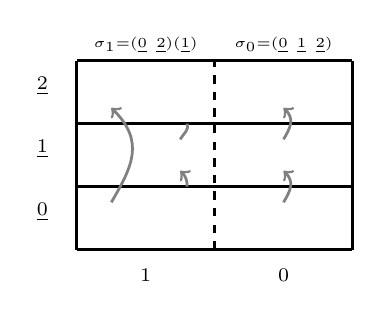
\begin{tikzpicture}[yscale=.8, xscale=1.75, line width=1pt ]
    % Linien.
    \foreach \i in {0,...,3}
    {
        \draw[color=black] (0,\i) -- (2,\i);
    }
    \draw[color=black] (0,0) -- (0,3);
    \draw[color=black, dashed] (1,0) -- (1,3);
    \draw[color=black] (2,0) -- (2,3); 
    
    \draw[->, color=black!50] (1.5, 0.75) to[out=75, in=295] (1.5, 1.25);
    \draw[->, color=black!50] (1.5, 1.75) to[out=75, in=295] (1.5, 2.25);
    
    \draw[    color=black!50] (0.75, 1.75) to[out=75, in=280] (0.8 , 2   );
    \draw[->, color=black!50] (0.8 , 1   ) to[out=90, in=295] (0.75, 1.25);
    
    \draw[->, color=black!50] (0.25, 0.75) to[out=75, in=295] (0.25, 2.25);
    
    % Beschriftung.
    \draw node at (-.25,2.5) {$\scriptstyle\ul 2$};
    \draw node at (-.25,1.5) {$\scriptstyle\ul 1$};
    \draw node at (-.25,0.5) {$\scriptstyle\ul 0$};
    
    \draw node at (0.5,-.4) {$\scriptstyle 1$};
    \draw node at (1.5,-.4) {$\scriptstyle 0$};
    
    \draw node at (0.5,3.25) {$\scriptscriptstyle\sigma_1 = (\ul0\ \ul2)(\ul1)$};
    \draw node at (1.5,3.25) {$\scriptscriptstyle\sigma_0 = (\ul0\ \ul1\ \ul2)$};
\end{tikzpicture}
\end{minipage}
\hspace{.5cm}
\begin{minipage}{.35\textwidth}
\centering
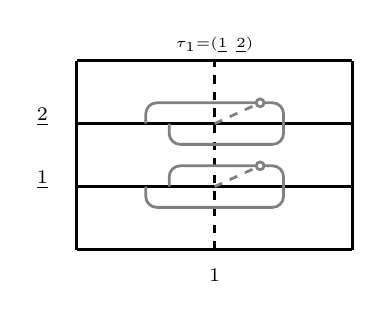
\begin{tikzpicture}[yscale=.8, xscale=1.75, line width=1pt ]
    % Linien.
    \foreach \i in {0,...,3}
    {
        \draw[color=black] (0,\i) -- (2,\i);
    }
    \draw[color=black] (0,0) -- (0,3);
    \draw[color=black, dashed] (1,0) -- (1,3);
    \draw[color=black] (2,0) -- (2,3); 
    
    \draw[color=gray, rounded corners] (0.67,1) -- (0.67,1.33) --  (1.5, 1.33) -- (1.5, 0.67) -- (0.5, 0.67) -- (0.5, 1);
    \draw[color=gray, rounded corners] (0.5,2) -- (0.5,2.33) --  (1.5, 2.33) -- (1.5, 1.67) -- (0.67, 1.67) -- (0.67, 2);
    
    \draw[color=gray, dashed] (1,1) -- (1.33, 1.33) node[fill=white, draw=gray, shape=circle, inner sep=1pt, solid] {};
    \draw[color=gray, dashed] (1,2) -- (1.33, 2.33) node[fill=white, draw=gray, shape=circle, inner sep=1pt, solid] {};
    
    % Beschriftung.
    \draw node at (-.25,2) {$\scriptstyle \ul 2$};
    \draw node at (-.25,1) {$\scriptstyle \ul 1$};
    
    \draw node at (1,-.4) {$\scriptstyle 1$};
    
    \draw node at (1,3.25) {$\scriptscriptstyle \tau_1 = (\ul1\ \ul2)$};
\end{tikzpicture}
\end{minipage}

\end{document}